\chapter{Approche}

\epigraph{<< Les plans sont inutiles, mais la planification est indispensable >>}{Dwight David Eisenhower}

En parallèle à nos différentes phases de planning (cf. figure \ref{pic:ganttChart}), nous devions nous appliquer à mettre en place une méthode de travail efficace. Que ce soit au niveau de notre binôme ou des meetings prévus chaque semaine avec nos deux promoteurs, il fallait trouver une manière de s'organiser afin de mener notre mémoire sur la bonne voie. Ce chapitre a donc pour but d'expliquer notre méthodologie de travail (méthode utilisée, phases du travail, communication), l'élaboration d'un planning et l'organisation du travail en interne.

\section{Méthodologie}
\label{section:methodologie}

De par la nature ouverte du projet à accueillir continuellement des nouvelles fonctionnalités et changements, une méthode Agile a été plébiscitée (qui s'oppose aux méthodes classiques plus rigides comme \textit{waterfall}). Comme expliqué par le manifeste Agile\cite{agileManifeste}, un certain nombre de principes sont présents et nous n'évoquerons ici que les plus importants : 

\begin{description}
    \item[\textbf{Satisfaction du client avant tout}] Il s'agit du principe sacro-saint de la méthode Agile\cite{agileManifeste}. Au lieu d'avoir un planning bien ficelé, il faut accepter l'ajout de nouvelles fonctionnalités et des changements (même tardifs) pour viser ce but.
    
    \item[\textbf{Itérations courtes}] En méthode Agile\cite{agileManifeste}, il est préconisé d'adopter des cycles de développement de faible durée afin de notamment identifier et corriger très tôt des bugs (une expression anglophone y est dédiée : "fail fast, fail often"). Puisque nous rencontrions nos promoteurs à peu près toutes les semaines, c'est naturellement ce rythme qui s'est imposé pour nos itérations.
    
    \item[\textbf{Livraison continue}] Tout au long du projet, de nombreux utilisateurs dont nos promoteurs ont utilisé intensivement l'application et nous ont livré quantité d'avis et retours. Il était donc nécessaire de déployer des versions de l'application très régulièrement pour montrer son avancement et donner la possibilité d'essayer de nouvelles fonctionnalités par les utilisateurs : nous avons fini par automatiser une grande partie de ce processus (nous expliquerons en détail dans la section \ref{section:validation} comment cela a été réalisé concrètement).
\end{description}

\subsection*{Phases du travail}

Pouvoir baliser les grandes étapes de ce travail est indispensable, car cela permet de suivre en outre l'évolution générale tout au long de ce projet. Bien que l'étape de développement (implémentation) suive les principes d'une méthode Agile\cite{agileManifeste}, il est inévitable de passer par les différentes étapes du développement logiciel (analyse, conception, implémentation, validation et déploiement). \\
% TODO glossaire déploiement ? (link avec Docker)

Ceci a été motivé par de multiples raisons. On citera notamment le vaste contexte très ouvert de la recherche et référencement des \glspl{resinfo}, pour laquelle il a fallu accorder une période de réflexion et d'analyse assez conséquente. \\

Un autre facteur a été que de nouveaux besoins et idées ont émergé au fur et à mesure de la construction de notre solution/prototype. Ces circonstances nous ont donc contraints à revoir constamment notre approche et notre organisation. 
Une manière de l'illustrer est de considérer la phase de validation (cf. section \ref{section:validation}), consistant à certifier que la solution ainsi développée correspond bien aux critères techniques qu'aux critères de satisfaction client. Le versionnage (c.-à-d. le fait de gérer plusieurs versions) de notre solution/prototype a permis de récolter de précieux retours d'utilisateurs au plus vite, tout en permettant d'identifier d'éventuelles régressions entre une version et une autre. \\

\subsection*{Communication}

En méthode Agile\cite{agileManifeste}, il y a de manière générale 2 questions récurrentes, et ce peu importe la taille et la nature des projets :
\begin{itemize}
    \item Où on en est ? 
    \begin{itemize}
        \item À quelle vitesse on progresse ?
        \item Qu'avons-nous réalisé ?
    \end{itemize}
    \item Quand on délivre le produit ?
    \begin{itemize}
        \item Que reste-t-il à faire ?
        \item Comment estimer le temps/travail nécessaire pour réaliser les différentes tâches ?
    \end{itemize}
\end{itemize}

Pour y répondre, il convient d'utiliser des moyens/outils de communication suffisamment explicites pour tous les acteurs de ce projet. Étant donné que notre solution est hébergée sur Github, nous avons décidé d'utiliser les fonctionnalités suivantes de Github : le "Project Board" \footnote{\url{https://help.github.com/en/github/managing-your-work-on-github/about-project-boards}} et les issues \footnote{\url{https://help.github.com/en/github/managing-your-work-on-github/about-issues}}. (dont vous pourrez trouver une illustration respectivement aux figures \ref{pic:GithubBoard} et \ref{pic:GithubIssues})\\

Comme nous pouvons le voir, par l'usage de ces outils/moyens, l'état et la progression générale du projet sont accessibles au plus grand nombre : 
\begin{itemize}
    \item Avec le "Project Board", on représente les tâches sous la forme de cartes amovibles dans un tableau, avec les caractéristiques suivantes :
    \begin{itemize}
        \item Chaque tâche est catégorisée dans une colonne bien précise ("to do"/ à réaliser, "in progress"/ en cours, "done" / réalisée, "enhancements" / améliorations)
        \item Une barre de progression nous notifie de l'avancement général du projet
    \end{itemize}
    \item Avec les issues (figure \ref{pic:GithubIssues}), chaque tâche/problème dispose des éléments suivants : 
    \begin{itemize}
        \item un titre pour expliquer brièvement celle-ci
        \item une étiquette en couleur pour notifier sa nature (problème, amélioration, documentation, etc.)
        \item la personne assignée sur celle-ci
        \item le statut de celle-ci (ouverte/fermée)
    \end{itemize}
\end{itemize}


\begin{figure}[H]
    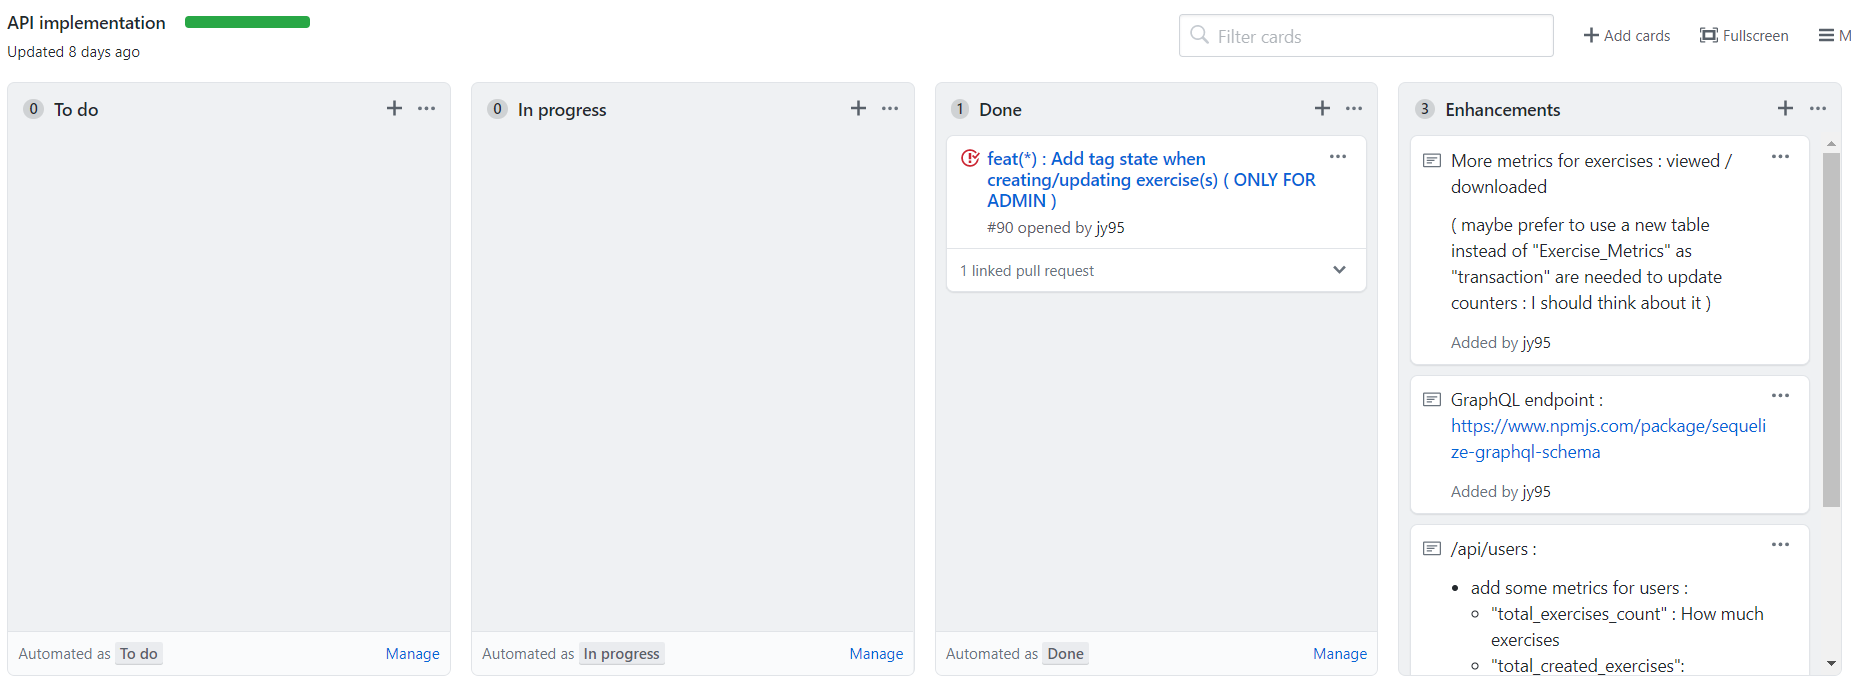
\includegraphics[width=\textwidth,height=\textheight,keepaspectratio]{images/approche/trelloLike.PNG}
    \centering
    \caption{Exemple d'interface Github Project Board}
    \label{pic:GithubBoard}
\end{figure}

\begin{figure}[H]
    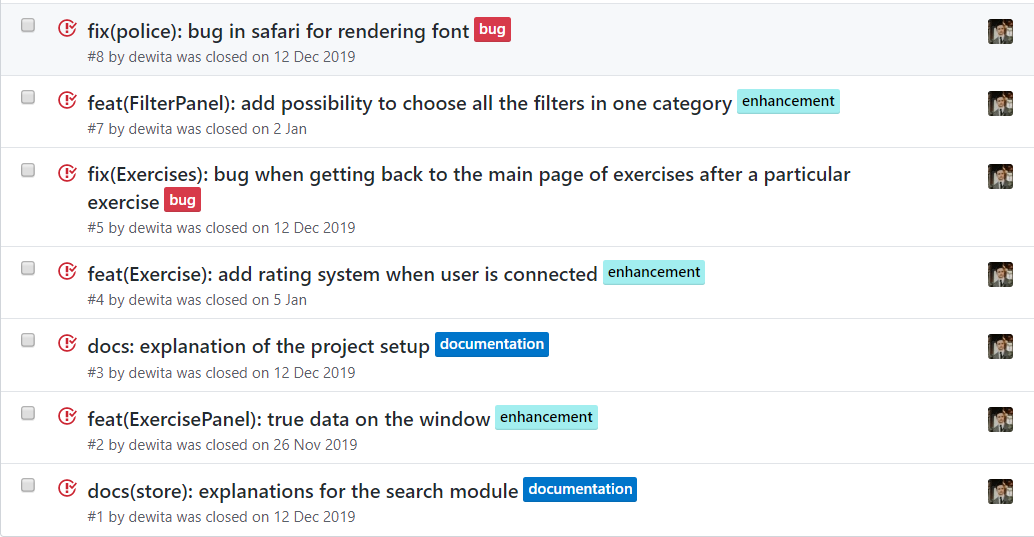
\includegraphics[width=\textwidth,height=\textheight,keepaspectratio]{images/approche/issueList.PNG}
    \centering
    \caption{Exemple d'issues sur Github}
    \label{pic:GithubIssues}
\end{figure}

\section{Planning}
Comme illustré par la citation en tête de ce chapitre, avoir un planning est plus utile qu'avoir un plan bien ficelé, car de nombreux obstacles imprévus peuvent nuire à celui-ci (dont nous avons cité quelques-unes au point  \ref{section:methodologie})\\

Vous pourrez retrouver ci-dessous une représentation simplifiée du diagramme de Gantt\footnote{Un diagramme de Gantt permet de représenter en outre la planification des diverses tâches du projet en fonction du temps } finale sous la forme d'une ligne du temps sur laquelle sont placées les grandes étapes du projet ainsi que les deux versions majeures (alpha et beta) que nous avons présentées aux différents acteurs du projet.\\

\begin{figure}[H]
    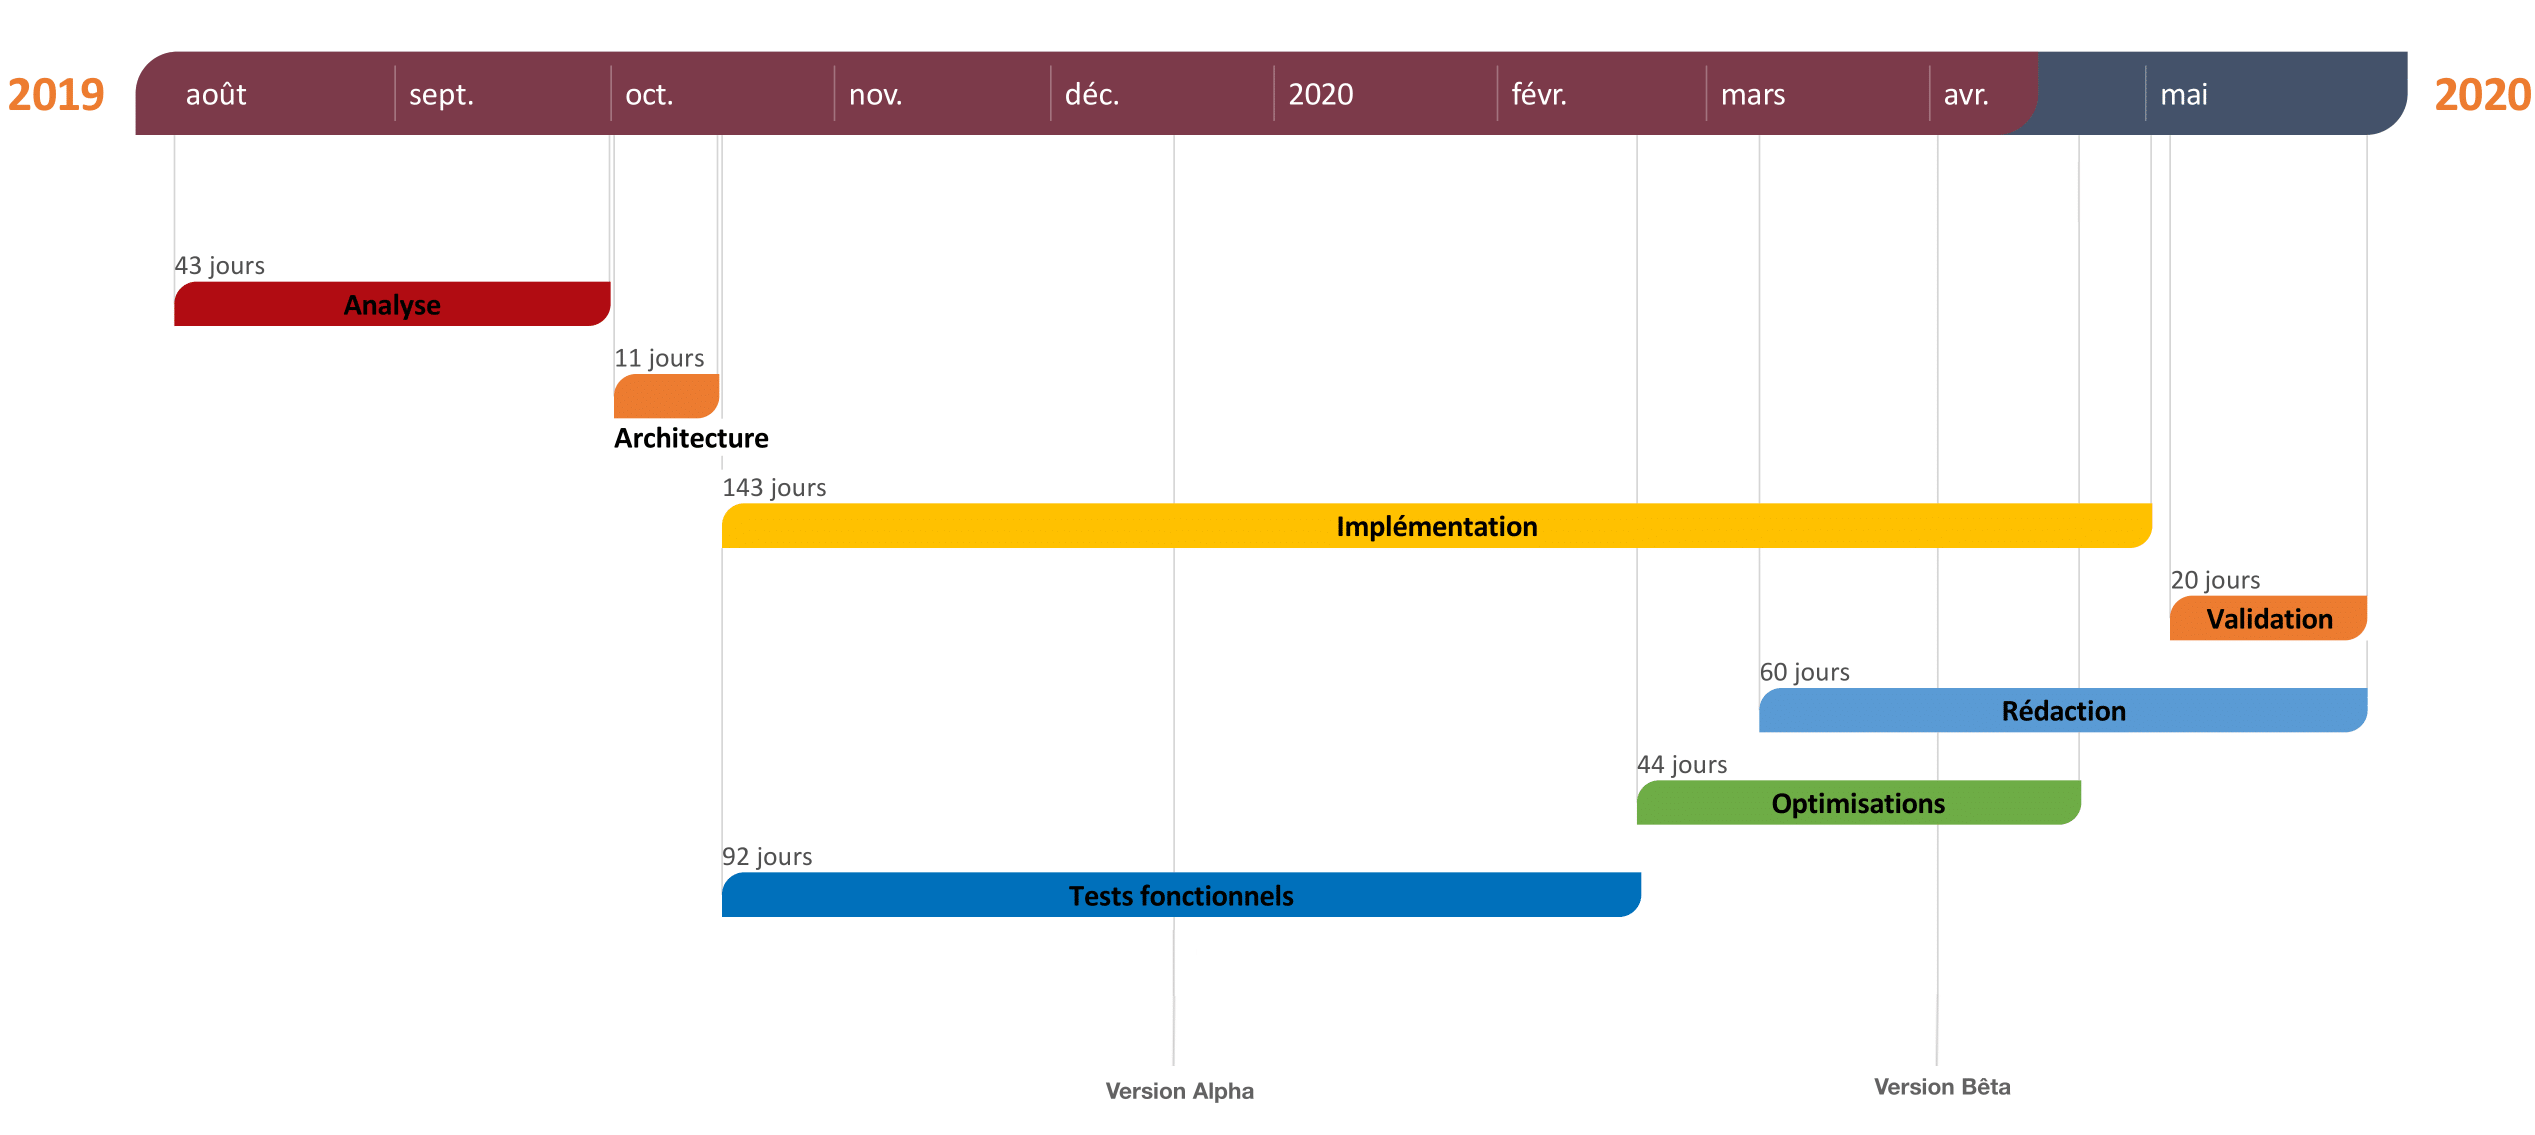
\includegraphics[width=\textwidth,height=\textheight,keepaspectratio]{images/approche/planning.png}
    \centering
    \caption{Diagramme de Gantt simplifié}
    \label{pic:ganttChart}
\end{figure}

Comparé au plan initial, on note des changements plus ou moins conséquents. Il était prévu d'accorder plus de temps aux phases primaires du projet (analyse et conception) pour partir sur de bonnes bases. Cela s'est avéré impossible tant l'usage de données concrètes dans nos ébauches semblait indispensable pour avoir des retours constructifs sur notre solution au plus tôt. De nombreuses fonctionnalités ont été rajoutées au fur et à mesure de l'avancement du projet, ce qui a prolongé la phase d'implémentation jusqu'au mois d'avril (sans oublier son démarrage précoce en octobre). \\

Fort heureusement, le démarrage très précoce du projet nous a permis de surmonter les nombreux obstacles et imprévus (grâce à notre méthodologie expliquée à la section \ref{section:methodologie}) sur notre chemin et de réaliser la majorité des tâches initialement prévues ainsi qu'une part conséquente des suggestions apportées tout au long du projet. \\

% TODO Ce serait bien de les détailler et d'expliquer quels catégories de problèmes vous avez eu et comment vous les avez résolu

\section{Organisation du travail}

Dès le départ, nous avons tiré à notre avantage les capacités et centres d'intérêt de chaque membre de notre groupe. Par chance, la complémentarité de notre duo a été telle que la répartition des tâches n'a pas posé de soucis, sans oublier une aide mutuelle en cas de besoin. Dans cette section, nous aborderons notre organisation et ses implications lors des différentes étapes de ce travail.\\

\subsection*{Analyse}

Cette phase consistait en ces 3 actions fondamentales :
\begin{itemize}
    \item Effectuer des recherches bibliographiques concernant l'étiquetage de \glspl{resinfo} (dont vous pouvez consulter la synthèse de celle-ci en annexe \ref{annexe:AnalyseBiblio}).
    \item Étudier des solutions similaires, présentes sur le web (que nous avons consigné en table \ref{table:compPlateforme}) pour en dresser les forces et faiblesses de chacune d'entre elles.
    \item Formaliser les besoins (exprimés en section \ref{section:challengesToDefeat}) en fonctionnalités.
\end{itemize}

De par sa nature essentielle, chaque membre de notre équipe a été impliqué dans l'analyse. Si cette étape s'est principalement déroulée d'août à fin septembre, il a été nécessaire de réaliser régulièrement des phases d'analyses complémentaires pour compléter ou réaliser des fonctionnalités.

\subsection*{Conception et implémentation}

Contrairement à l'analyse, la conception et l'implémentation ont été réalisées en fonction du domaine spécifique de chacun : 

\begin{description}
    \item[Jacques] : responsable du \gls{backend} et du \Gls{cli} : base de données, extraction et nettoyage des données, gestion de la performance et la sécurité.
    \item[Alexandre] : responsable du \gls{frontend} : prototypage de l'application, interface graphique.
\end{description}

Le principal problème avec cette approche est la "compartimentation" qui favorise une connaissance limitée de la totalité des technologies utilisées. Ceci risque de provoquer un arrêt qui, temporairement ou non, nuit à la bonne réalisation de nos objectifs dans les délais fixés si un membre de notre équipe se retrouve dans l'incapacité sa part de travail pour l'une ou l'autre raison. \\

Une solution fréquemment utilisée en entreprise pour pallier ce problème est d'impliquer plus d'acteurs sur chaque partie du développement ou la totalité du code (avec un système d'affectation des tâches, rotatif ou non). \\

Ce choix n'en est pas dénoué d'avantages, car en outre de permettre une haute maîtrise des technologies utilisées dans chaque partie, on a un interlocuteur unique à qui poser des questions spécifiques.

\subsection*{Rédaction}


L'écriture de ce présent manuscrit a rassemblé l'ensemble de notre équipe. En tant que document qui représente l'aboutissement du travail commun accompli, la présence de chacun est indispensable dans sa réalisation. Dès le départ, nous avons accordé une grande importance à celui-ci lors de la planification du travail (représenté par la figure \ref{pic:ganttChart}), car l'ampleur de cette tâche ne s'improvise pas en dernière minute. \\

L'élaboration de ce document s'est faite par étapes. Tout d'abord, nous avons réalisé un plan de rédaction simplifiée consistant à représenter les divers sujets et points du contenu à aborder autour d'un fil rouge conducteur. Ensuite, un premier jet à réaliser a été attribué au mémorant des différentes parties sous sa responsabilité. Enfin, nous sommes passés par un laborieux processus répété de relecture et d'améliorations continues du texte, notamment orientés par les nombreux commentaires de nos promoteurs.